\chapter{Specifikacija programske potpore}

\section{Funkcionalni zahtjevi}

\noindent \textbf{Dionici:}

\begin{packed_enum}
	
	\item Administrator
	\item Organizatori događaja
	\item Građani (posjetitelji)
	\item Razvojni tim				
	
\end{packed_enum}

\noindent \textbf{Aktori i njihovi funkcionalni zahtjevi:}


\begin{packed_enum}
	\item  \underbar{Neregistrirani/neprijavljeni korisnik (inicijator) može:}
	
	\begin{packed_enum}
		\item pregledati stranicu \textit{O nama}
		\item stvoriti novi korisnički račun kao:
		\begin{packed_enum}
			\item organizator (korisničko ime, e-mail adresa, lozinka, adresa) 
			\item  posjetitelj (korisničko ime, e-mail adresa, lozinka) 
		\end{packed_enum} 
		\item prijaviti se u sustav
		
	\end{packed_enum}
	
	\item  \underbar{Posjetitelj (inicijator) može:}
	
	\begin{packed_enum}
		
		\item prijaviti se u sustav i odjaviti iz sustava
		\item pregledavati i uređivati svoje osobne podatke
		\item vidjeti popis aktualnih događanja u odabranom vremenskom razdoblju (24 sata, 7 dana, 30 dana)
		\item odabrati postavke da im aplikacija automatski šalje obavijesti o najnovijim događanjima (prema vrsti događanja i području) 
		\item za svako događanje: 
		\begin{packed_enum}
			\item iskazati interes (\textit{sigurno dolazim, možda dolazim, ne dolazim})
			\item po želji promijeniti interes
		\end{packed_enum} 
		\item vidjeti podatke o organizatorima događanja (naziv, adresa, poveznica na vlastite web ili Facebook stranice,  popis svih događanja koja su oglašena putem aplikacije u zadnje 2 godine)
		\item napisati recenziju (i/ili obrisati svoju napisanu recenziju) za događanja koja su završila u posljednjih 48 sati
		\item obrisati svoj korisnički račun
		\item odjaviti se iz sustava
		
	\end{packed_enum}
	
	\item \underbar{Organizator (inicijator) može:}		
	
	\begin{packed_enum}
		\item sve što može i Posjetitelj
		\item unošenjem obaveznih i, po želji, opcionalnih podataka, ovisno plaća li članarinu, stvoriti novo događanje:
		\begin{packed_enum}
			\item za koje se ne plaća ulaz 
			\item za koje se plaća ulaz ili za koje se ne plaća ulaz
		\end{packed_enum}
		\item pregledavati i brisati svoja događanja 
	\end{packed_enum}
	
	\item \underbar{Administrator (inicijator) može:}
	
	\begin{packed_enum}
		\item prijaviti se u sustav
		\item vidjeti popis i osobne podatke svih registriranih korisnika 
		\item trajno obrisati korisnički profil
		\item postaviti cijenu članarine za organizatore događanja za koje se plaća ulaz
		\item brisati recenzije i događanja 
		\item odjaviti se iz sustava
	\end{packed_enum}
	
	\item \underbar{Baza podataka (sudionik):}
	\begin{packed_enum}
		\item pohranjuje podatke registriranih korisnika 
		\item pohranjuje podatke o događanjima 
		\item pohranjuje recenzije događanja 
	\end{packed_enum}
\end{packed_enum}

\eject 



\subsection{Obrasci uporabe}

\subsubsection{Opis obrazaca uporabe}

\noindent U nastavku su detaljno opisani obrasci upotrebe označenih kraticom UC i rednim brojem obrasca. Obrasci predstavljaju ključne scenarije interakcije između korisnika i samog sustava. Svaki UC pruža jasno strukturirane korake koje korisnik slijedi i omogućuje razumijevanje odziva sustava na te korake.  \\

\noindent \underbar{\textbf{UC1 - Pregled stranice O nama}}
\begin{packed_item}
	
	\item \textbf{Glavni sudionik:} Neregistrirani/neprijavljeni korisnik i prijavljeni korisnik
	\item  \textbf{Cilj:} Pregled stranice s općim informacijama o web aplikaciji
	\item  \textbf{Sudionici:} -
	\item  \textbf{Preduvjet:} -
	\item  \textbf{Opis osnovnog tijeka:}
	
	\item[] \begin{packed_enum}
		
		\item Korisnik odabire opciju prikaza stranice O nama
		\item Otvara se stranica i prikazuju informacije o web aplikaciji
		
	\end{packed_enum}						
\end{packed_item}


%	%	%	%	%	%	%	%	%	%	%	%	%	%	%	%	%					

\noindent \underbar{\textbf{UC2 - Registracija}}
\begin{packed_item}
	
	\item \textbf{Glavni sudionik:} Neregistrirani/neprijavljeni korisnik
	\item  \textbf{Cilj:} Stvaranje korisničkog računa za korištenje platforme
	\item  \textbf{Sudionici:} Baza podataka
	\item  \textbf{Preduvjet:} -
	\item  \textbf{Opis osnovnog tijeka:}
	
	\item[] \begin{packed_enum}
		
		\item Korisnik odabire opciju registracije
		\item Korisnik unosi tražene podatke 
		\item Baza podataka se osvježava
		\item Korisnik dobiva pristup korisničkim funkcijama i obavijest o uspješnoj registraciji te se preusmjerava na početnu stranicu za prijavljene korisnike 
		
	\end{packed_enum}
	
	\item  \textbf{Opis mogućih odstupanja:}
	
	\item[] \begin{packed_item}
		
		\item[2.a] Uneseno zauzeto korisničko ime i/ili e-mail adresa, korisničko ime i/ili lozinka u nedozvoljenom formatu, neispravna e-mail adresa 
		\item[] \begin{packed_enum}
			
			\item Obavijestiti korisnika o neispravnom unosu i omogućiti ponovni unos neprihvaćenih vrijednosti
			\item Korisnik unosi nove vrijednosti i uspješno završava registraciju ili odustaje od registracije 
			
		\end{packed_enum}
	\end{packed_item}
	
\end{packed_item}

%	%	%	%	%	%	%	%	%	%	%	%	%	%	%	%	%	%	%

\newpage

\noindent \underbar{\textbf{UC3 - Prijava}}
\begin{packed_item}
	
	\item \textbf{Glavni sudionik:} Neregistrirani/neprijavljeni korisnik
	\item  \textbf{Cilj:} Dobiti pristup odgovarajućem korisničkom sučelju ovisno o ulozi 
	\item  \textbf{Sudionici:} Baza podataka
	\item  \textbf{Preduvjet:} Registracija
	\item  \textbf{Opis osnovnog tijeka:}
	
	\item[] \begin{packed_enum}
		
		\item Korisnik odabire opciju prijave u sustav
		\item Korisnik unosi tražene podatke (korisničko ime i lozinka)
		\item Provjera ispravnosti unesenih podataka 
		\item Korisnik dobiva obavijest o uspješnoj prijavi i preusmjerava se na početnu stranicu za prijavljene korisnike 
		
	\end{packed_enum}
	
	\item  \textbf{Opis mogućih odstupanja:}
	
	\item[] \begin{packed_item}
		
		\item[2.a] Uneseno neispravno korisničko ime i/ili lozinka  
		\item[] \begin{packed_enum}
			
			\item Obavijestiti korisnika o neuspješnoj registraciji i omogućiti ponovni unos korisničkog imena i/ili lozinke
			\item Korisnik unosi nove vrijednosti i uspješno se prijavljuje ili odustaje od prijave
			
		\end{packed_enum}
	\end{packed_item}
	
\end{packed_item}

%	%	%	%	%	%	%	%	%	%	%	%	%	%	%	%	%	%	%


\noindent \underbar{\textbf{UC4 - Odjava}}
\begin{packed_item}
	
	\item \textbf{Glavni sudionik:} Prijavljeni korisnik (Administrator, Organizator, Posjetitelj)
	\item  \textbf{Cilj:} Odjava iz sustava 
	\item  \textbf{Sudionici:} -
	\item  \textbf{Preduvjet:} Korisnik je trenutno prijavljen u sustav
	\item  \textbf{Opis osnovnog tijeka:}
	
	\item[] \begin{packed_enum}
		
		\item Korisnik odabire opciju odjave
		\item Korisnik gubi pristup korisničkim funkcijama
		\item Korisnik se preusmjerava na početnu stranicu za neregistrirane/neprijavljene korisnike 
		
	\end{packed_enum}
\end{packed_item}

%	%	%	%	%	%	%	%	%	%	%	%	%	%	%	%	%	%	%

\noindent \underbar{\textbf{UC5 - Pregled osobnih podataka}}
\begin{packed_item}
	
	\item \textbf{Glavni sudionik:} Korisnik (Organizator, Posjetitelj)
	\item  \textbf{Cilj:} Pregledati osobne podatke
	\item  \textbf{Sudionici:} Baza podataka
	\item  \textbf{Preduvjet:} Korisnik je trenutno prijavljen u sustav
	\item  \textbf{Opis osnovnog tijeka:}
	
	\item[] \begin{packed_enum}
		
		\item Korisnik odabire opciju za pregled svog profila
		\item Prikazuju se osobni podaci vezani uz korisnički račun
		
	\end{packed_enum}
\end{packed_item}

%	%	%	%	%	%	%	%	%	%	%	%	%	%	%	%	%	%	%

\noindent \underbar{\textbf{UC6 - Uređivanje osobnih podataka}}
\begin{packed_item}
	
	\item \textbf{Glavni sudionik:} Korisnik (Organizator, Posjetitelj)
	\item  \textbf{Cilj:} Izmijeniti osobne podatke 
	\item  \textbf{Sudionici:} Baza podataka
	\item  \textbf{Preduvjet:} Korisnik je trenutno prijavljen u sustav
	\item  \textbf{Opis osnovnog tijeka:}
	
	\item[] \begin{packed_enum}
		
		\item Korisnik odabire opciju izmjene osobnih podataka
		\item Korisnik mijenja željene podatke 
		\item Provjera ispravnosti unesenih podataka 
		\item Korisnik sprema promjene
		\item Baza podataka se osvježava 
		
	\end{packed_enum}
	
	\item  \textbf{Opis mogućih odstupanja:}
	
	\item[] \begin{packed_item}
		
		\item[2.a] Novo uneseni podaci su nedozvoljene vrijednosti
		\item[] \begin{packed_enum}
			
			\item Onemogućiti spremanje promjena
			\item Obavijestiti korisnika o nedozvoljenim vrijednostima i omogućiti ponovni unos 
			\item Korisnik unosi nove vrijednosti i omogućava se spremanje promjena
			
		\end{packed_enum}
		
		\item[4.a] Korisnik pokušava napustiti prozor, a nije spremio promjene 
		\item[] \begin{packed_enum}
			
			\item Obavijestiti korisnika o obaveznom spremanju promjena
			\item Nakon spremanja promjena omogućiti izlaz iz prozora
			
		\end{packed_enum}
		
	\end{packed_item}
	
\end{packed_item}

%	%	%	%	%	%	%	%	%	%	%	%	%	%	%	%	%	%	%

\noindent \underbar{\textbf{UC7 - Postavke obavještavanja o novim događanjima}}
\begin{packed_item}
	
	\item \textbf{Glavni sudionik:} Prijavljeni korisnik (Organizator, Posjetitelj)
	\item  \textbf{Cilj:} Podesiti postavke obavještavanja o najnovijim događanjima
	\item  \textbf{Sudionici:} Baza podataka
	\item  \textbf{Preduvjet:} Korisnik je trenutno prijavljen u sustav i ima ovlasti Posjetitelja
	\item  \textbf{Opis osnovnog tijeka:}
	
	\item[] \begin{packed_enum}
		
		\item Korisnik odabire opciju uređivanja postavki obavještavanja o novim događanjima
		\item Korisnik odabire želi li primati obavijesti i, ako da, o kojim vrstama događanja i na kojem području
		\item Korisnik sprema promjene
		\item Baza podataka se osvježava
		
	\end{packed_enum}
	
	%\item  \textbf{Opis mogućih odstupanja:}
	
	%\item[] \begin{packed_item}
		
		%	\item[2.a] Korisnik odabire da želi primati obavijesti, ali ne unese minimalno jednu vrstu događanja i minimalno jedno područje
		%	\item[] \begin{packed_enum}
			
			%		\item Onemogućiti spremanje promjena
			%		\item Obavijestiti korisnika o obaveznom izboru barem jedne vrste događanja i barem jednog područja
			%		\item Korisnik odabire vrstu događanja i/ili područje koje nedostaje i omogućava se spremanje promjena
			
			%	\end{packed_enum}
		%\end{packed_item}
		
	\end{packed_item}
	
	%	%	%	%	%	%	%	%	%	%	%	%	%	%	%	%	%	%	%
	
	\noindent \underbar{\textbf{UC8 - Brisanje vlastitog korisničkog računa}}
	\begin{packed_item}
		
		\item \textbf{Glavni sudionik:} Korisnik (Organizator, Posjetitelj)
		\item  \textbf{Cilj:} Obrisati korisnički račun i sve osobne podatke
		\item  \textbf{Sudionici:} Baza podataka
		\item  \textbf{Preduvjet:} Korisnik je trenutno prijavljen u sustav i otvoren je pregled osobnih podataka
		\item  \textbf{Opis osnovnog tijeka:}
		
		\item[] \begin{packed_enum}
			
			\item Korisnik odabire opciju brisanja korisničkog računa
			\item Korisnik potvrđuje svoj odabir 
			\item Baza podataka se osvježava
			\item Korisnik se preusmjerava na početnu stranicu za neregistrirane/neprijavljene korisnike 
			
		\end{packed_enum}
		
	\end{packed_item}
	
	%	%	%	%	%	%	%	%	%	%	%	%	%	%	%	%	%	%	%
	
	
	\noindent \underbar{\textbf{UC9 - Pregled svih korisničkih računa}}
	\begin{packed_item}
		
		\item \textbf{Glavni sudionik:} Administrator
		\item  \textbf{Cilj:} Prikaz svih korisničkih računa 
		\item  \textbf{Sudionici:} Baza podataka
		\item  \textbf{Preduvjet:} Korisnik je trenutno prijavljen u sustav i ima ovlasti Administratora
		\item  \textbf{Opis osnovnog tijeka:}
		
		\item[] \begin{packed_enum}
			
			\item Administrator odabire opciju pregleda korisničkih računa
			\item Prikazuje se popis svih korisničkih računa
			
		\end{packed_enum}
		
	\end{packed_item}
	
	%	%	%	%	%	%	%	%	%	%	%	%	%	%	%	%	%	%	%
	
	\noindent \underbar{\textbf{UC10 - Brisanje korisničkog računa}}
	\begin{packed_item}
		
		\item \textbf{Glavni sudionik:} Administrator
		\item  \textbf{Cilj:} Trajno brisanje korisnika iz sustava
		\item  \textbf{Sudionici:} Baza podataka
		\item  \textbf{Preduvjet:} Korisnik je prijavljen, ima ovlasti Administratora i prikazan mu je popis svih korisničkih računa (\textbf{UC9})
		\item  \textbf{Opis osnovnog tijeka:}
		
		\item[] \begin{packed_enum}
			
			\item Administrator odabire opciju brisanja korisničkog računa 
			\item Administrator potvrđuje svoj odabir
			\item Baza podataka se osvježava
			\item Promjena je vidljiva u prikazanom popisu korisničkih računa
			
		\end{packed_enum}
		
	\end{packed_item}
	
	%	%	%	%	%	%	%	%	%	%	%	%	%	%	%	%	%	%	%
	
	\newpage
	
	\noindent \underbar{\textbf{UC11 - Postavljanje cijene članarine}}
	\begin{packed_item}
		
		\item \textbf{Glavni sudionik:} Administrator
		\item  \textbf{Cilj:} Postavljanje cijene mjesečne članarine za organizatore
		\item  \textbf{Sudionici:} Baza podataka
		\item  \textbf{Preduvjet:} Korisnik je prijavljen i ima ovlasti Administratora 
		\item  \textbf{Opis osnovnog tijeka:}
		
		\item[] \begin{packed_enum}
			
			\item Administrator odabire opciju postavljanja članarine
			\item Administrator unosi cijenu i sprema ju
			\item Baza podataka se osvježava
			
		\end{packed_enum}
		
		\item  \textbf{Opis mogućih odstupanja:}
		
		\item[] \begin{packed_item}
			
			\item[2.a] Unesena cijena nije ispravnog formata
			\item[] \begin{packed_enum}
				
				\item Onemogućiti spremanje promjena
				\item Obavijestiti korisnika o nedozvoljenoj vrijednosti i omogućiti ponovni unos 
				\item Korisnik unosi novu vrijednost i omogućava se spremanje promjena
				
			\end{packed_enum}
		\end{packed_item}
		
	\end{packed_item}
	
	%	%	%	%	%	%	%	%	%	%	%	%	%	%	%	%	%	%	%
	
	\noindent \underbar{\textbf{UC12 - Dodavanje novog događanja}}
	\begin{packed_item}
		
		\item \textbf{Glavni sudionik:} Organizator
		\item  \textbf{Cilj:} Dodati novo događanje 
		\item  \textbf{Sudionici:} Baza podataka
		\item  \textbf{Preduvjet:} Korisnik je prijavljen i ima ovlasti Organizatora
		\item  \textbf{Opis osnovnog tijeka:}
		
		\item[] \begin{packed_enum}
			
			\item Organizator odabire opciju dodavanja novog događanja
			\item Organizator upisuje potrebne i, po želji, opcionalne podatke o događanju (naziv, vrsta, lokacija, vrijeme početka, trajanje, cijena; opcionalno fotografije, videozapisi)
			
			\item Ovisno o tome ima li Organizator mogućnost organiziranja događanja koja se plaćaju: 
			\item[] \begin{packed_enum}
				\item ako ima, Organizator bira plaća li se ili ne novo događanje koje dodaje 
				\item ako nema mogućnost organiziranja događanja koja se plaćaju, podrazumijeva se da je događanje besplatno
			\end{packed_enum}
			
			\item Organizator dovršava objavu i objavljuje ju
			\item Baza podataka se osvježava
			\item Događanje će biti prikazano na stranici
			
		\end{packed_enum}
		
		\item  \textbf{Opis mogućih odstupanja:}
		
		\item[] \begin{packed_item}
			
			\item[2.a] Uneseni podaci su nedozvoljene vrijednosti
			\item[] \begin{packed_enum}
				
				\item Onemogućiti završetak dodavanja događanja
				\item Obavijestiti korisnika o nedozvoljenim vrijednostima i omogućiti ponovni unos 
				\item Korisnik unosi nove vrijednosti i omogućava se nastavak na objavu događanja
				
			\end{packed_enum}		
		\end{packed_item}
		
	\end{packed_item}
	
	%	%	%	%	%	%	%	%	%	%	%	%	%	%	%	%	%	%	%
	
	\noindent \underbar{\textbf{UC13 - Pregled svih događanja}}
	\begin{packed_item}
		
		\item \textbf{Glavni sudionik:} Prijavljeni korisnik (Posjetitelj, Organizator, Administrator)
		\item  \textbf{Cilj:} Pregled svih događanja prema određenom kriteriju
		\item  \textbf{Sudionici:} Baza podataka
		\item  \textbf{Preduvjet:} Korisnik je trenutno prijavljen u sustav 
		\item  \textbf{Opis osnovnog tijeka:}
		
		\item[] \begin{packed_enum}
			
			\item Na stranici s događanjima korisnik odabire kriterij prema kojem se prikazuju događanja (prikaz događanja završenih u zadnjih 48 sati ili aktualna događanja u narednih 24 sata, 7 dana, 30 dana)
			\item Događanja koja zadovoljavaju odabrani kriterij prikazuju se na stranici
			
		\end{packed_enum}
		
	\end{packed_item}
	
	%	%	%	%	%	%	%	%	%	%	%	%	%	%	%	%	%	%	%
	
	\noindent \underbar{\textbf{UC14 - Pregled jednog događanja}}
	\begin{packed_item}
		
		\item \textbf{Glavni sudionik:} Prijavljeni korisnik (Posjetitelj, Organizator, Administrator)
		\item  \textbf{Cilj:} Pregled jednog odabranog događanja od svih prikazanih događanja 
		\item  \textbf{Sudionici:} Baza podataka
		\item  \textbf{Preduvjet:} Korisnik je trenutno prijavljen u sustav i prikazana su sva događanja prema odabranom kriteriju (\textbf{UC13})
		\item  \textbf{Opis osnovnog tijeka:}
		
		\item[] \begin{packed_enum}
			
			\item Korisnik odabire jedno od prikazanih događanja
			\item Na zasebnoj se stranici korisniku prikazuju detalji o odabranom događanju
			
		\end{packed_enum}
		
	\end{packed_item}
	
	%	%	%	%	%	%	%	%	%	%	%	%	%	%	%	%	%	%	%				
	
	\noindent \underbar{\textbf{UC15 - Pregled profila organizatora}}
	\begin{packed_item}
		
		\item \textbf{Glavni sudionik:} Prijavljeni korisnik (Posjetitelj, Organizator)
		\item  \textbf{Cilj:} Pregled korisničkog računa organizatora
		\item  \textbf{Sudionici:} Baza podataka
		\item  \textbf{Preduvjet:} Korisnik je trenutno prijavljen u sustav, ima ovlasti Posjetitelja ili Organizatora i ima otvoren prikaz nekog događanja
		\item  \textbf{Opis osnovnog tijeka:}
		
		\item[] \begin{packed_enum}
			
			\item Posjetitelj odabire opciju prikaza profila organizatora
			\item Prikazuju se informacije o organizatoru
			
		\end{packed_enum}
		
	\end{packed_item}
	
	%	%	%	%	%	%	%	%	%	%	%	%	%	%	%	%	%	%	%
	
	\noindent \underbar{\textbf{UC16 - Pregled vlastitih događanja}}
	\begin{packed_item}
		
		\item \textbf{Glavni sudionik:} Organizator
		\item  \textbf{Cilj:} Pregled svih događanja koje je taj organizator objavio
		\item  \textbf{Sudionici:} Baza podataka
		\item  \textbf{Preduvjet:} Korisnik je trenutno prijavljen u sustav i ima ovlasti Organizatora  
		\item  \textbf{Opis osnovnog tijeka:}
		
		\item[] \begin{packed_enum}
			
			\item Organizator odabire opciju prikaza vlastitih događanja
			\item Ovisno o tome ima li organizator objavljenih događanja prikazuju se događanja ili odgovarajuća poruka
			
		\end{packed_enum}
		
	\end{packed_item}
	
	%	%	%	%	%	%	%	%	%	%	%	%	%	%	%	%	%	%	%
	
	\noindent \underbar{\textbf{UC17 - Pregled jednog vlastitog događanja}}
	\begin{packed_item}
		
		\item \textbf{Glavni sudionik:} Organizator
		\item  \textbf{Cilj:} Prikaz jednog od događanja koje je taj organizator objavio
		\item  \textbf{Sudionici:} Baza podataka
		\item  \textbf{Preduvjet:} Korisnik je trenutno prijavljen u sustav, ima ovlasti Organizatora i prikazana su mu sva vlastita događanja
		\item  \textbf{Opis osnovnog tijeka:}
		
		\item[] \begin{packed_enum}
			
			\item Organizator odabire opciju prikaza jednog od događanja
			\item Na zasebnoj se stranici organizatoru prikazuju detalji o odabranom događaju (uključujući i recenzije posjetitelja)
			
		\end{packed_enum}
		
	\end{packed_item}
	
	%	%	%	%	%	%	%	%	%	%	%	%	%	%	%	%	%	%	%
	
	\noindent \underbar{\textbf{UC18 - Brisanje vlastitog događanja}}
	\begin{packed_item}
		
		\item \textbf{Glavni sudionik:} Organizator
		\item  \textbf{Cilj:} Trajno brisanje vlastitog događanja
		\item  \textbf{Sudionici:} Baza podataka
		\item  \textbf{Preduvjet:} Korisnik je prijavljen, ima ovlasti Organizatora i prikazana su mu sva vlastita događanja
		\item  \textbf{Opis osnovnog tijeka:}
		
		\item[] \begin{packed_enum}
			
			\item Organizator odabire opciju brisanja događanja
			\item Organizator potvrđuje svoj odabir
			\item Baza podataka se osvježava
			\item Promjena je vidljiva u prikazanom popisu događanja
			
		\end{packed_enum}
		
	\end{packed_item}
	
	%	%	%	%	%	%	%	%	%	%	%	%	%	%	%	%	%	%	%
	
	\noindent \underbar{\textbf{UC19 - Brisanje događanja}}
	\begin{packed_item}
		
		\item \textbf{Glavni sudionik:} Administrator
		\item  \textbf{Cilj:} Trajno brisanje događanja
		\item  \textbf{Sudionici:} Baza podataka
		\item  \textbf{Preduvjet:} Korisnik je prijavljen, ima ovlasti Administratora i prikazana su mu sva događanja
		\item  \textbf{Opis osnovnog tijeka:}
		
		\item[] \begin{packed_enum}
			
			\item Administrator odabire opciju brisanja događanja
			\item Administrator potvrđuje svoj odabir
			\item Baza podataka se osvježava
			\item Promjena je vidljiva u prikazanom popisu događanja
			
		\end{packed_enum}
		
	\end{packed_item}
	
	%	%	%	%	%	%	%	%	%	%	%	%	%	%	%	%	%	%	%
	
	\noindent \underbar{\textbf{UC20 - Recenziranje događanja}}
	\begin{packed_item}
		
		\item \textbf{Glavni sudionik:} Prijavljeni korisnik (Organizator, Posjetitelj)
		\item  \textbf{Cilj:} Dodavanje recenzije događanja
		\item  \textbf{Sudionici:} Baza podataka
		\item  \textbf{Preduvjet:} Korisnik je prijavljen, ima ovlasti Posjetitelja ili Organizatora i otvoren je prikaz događanja koje je završilo u posljednjih 48 sati
		\item  \textbf{Opis osnovnog tijeka:}
		
		\item[] \begin{packed_enum}
			
			\item Posjetitelj odabire opciju dodavanja recenzije
			\item Posjetitelj upisuje ocjenu i recenziju događanja
			\item Posjetitelj potvrđuje da želi objaviti recenziju ili odustaje od objave
			\item Baza podataka se osvježava
			\item Recenzija je dodana i vidljiva na vrhu recenzija tog događanja
			
		\end{packed_enum}
		
		\item  \textbf{Opis mogućih odstupanja:}
		
		\item[] \begin{packed_item}
			
			\item[2.a] Recenzija nije napisana 
			\item[] \begin{packed_enum}
				
				\item Onemogućiti objavu recenzije 
				\item Posjetitelju omogućiti objavu recenzije ako i samo ako recenzija nije prazna, u protivnom posjetitelj odustaje od objave recenzije
				
			\end{packed_enum}		
		\end{packed_item}
		
	\end{packed_item}
	
	%	%	%	%	%	%	%	%	%	%	%	%	%	%	%	%	%	%	%
	
	\newpage
	
	\noindent \underbar{\textbf{UC21 - Brisanje vlastite recenzije}}
	\begin{packed_item}
		
		\item \textbf{Glavni sudionik:} Prijavljeni korisnik (Posjetitelj, Organizator)
		\item  \textbf{Cilj:} Trajno brisanje vlastite recenzije događanja
		\item  \textbf{Sudionici:} Baza podataka
		\item  \textbf{Preduvjet:} Korisnik je prijavljen, ima ovlasti Posjetitelja ili Organizatora i otvoren je prikaz jednog događanja
		\item  \textbf{Opis osnovnog tijeka:}
		
		\item[] \begin{packed_enum}
			
			\item Korisnik odabire opciju brisanja recenzije 
			\item Korisnik potvrđuje svoj odabir
			\item Baza podataka se osvježava
			\item Promjena je vidljiva u prikazanom događanju
			
		\end{packed_enum}
		
	\end{packed_item}
	
	%	%	%	%	%	%	%	%	%	%	%	%	%	%	%	%	%	%	%
	
	\noindent \underbar{\textbf{UC22 - Brisanje recenzije}}
	\begin{packed_item}
		
		\item \textbf{Glavni sudionik:} Administrator
		\item  \textbf{Cilj:} Trajno brisanje recenzije događanja
		\item  \textbf{Sudionici:} Baza podataka
		\item  \textbf{Preduvjet:} Korisnik je prijavljen, ima ovlasti Administratora i otvoren je prikaz jednog događanja
		\item  \textbf{Opis osnovnog tijeka:}
		
		\item[] \begin{packed_enum}
			
			\item Administrator odabire opciju brisanja recenzije 
			\item Administrator potvrđuje svoj odabir
			\item Baza podataka se osvježava
			\item Promjena je vidljiva u prikazanom događanju
			
		\end{packed_enum}
		
	\end{packed_item}
	
	%	%	%	%	%	%	%	%	%	%	%	%	%	%	%	%	%	%	%
	
	
	\noindent \underbar{\textbf{UC23 - Iskazivanje interesa za događanje}}
	\begin{packed_item}
		
		\item \textbf{Glavni sudionik:} Prijavljeni korisnik (Posjetitelj, Organizator)
		\item  \textbf{Cilj:} Izraziti i/ili promijeniti interes za događanje
		\item  \textbf{Sudionici:} Baza podataka
		\item  \textbf{Preduvjet:} Korisnik je trenutno prijavljen u sustav, ima ovlasti Posjetitelja ili Organizatora i otvoren je  prikaz nekog događanja 
		\item  \textbf{Opis osnovnog tijeka:}
		
		\item[] \begin{packed_enum}
			
			\item Posjetitelj odabire jednu od opcija \textit{sigurno dolazim, možda dolazim, ne dolazim }
			\item Eventualnim ponovnim pritiskom na opciju koja je odabrana poništava se taj odabir
			\item Baza podataka se osvježava
			\item Na prikazu tog događanja korisnik vidi svoj zadnji iskazani interes 
			
		\end{packed_enum}
		
		\item  \textbf{Opis mogućih odstupanja:}
		
		\item[] \begin{packed_item}
			
			\item[1.a] Posjetitelj odabire novu opciju, a jedna je već odabrana  
			\item[] \begin{packed_enum}
				
				\item Poništava se odabir koji je do tada vrijedio i bilježi se novi odabir
				
			\end{packed_enum}		
		\end{packed_item}
		
	\end{packed_item}
	
	
	
	\newpage
	
	
	\subsubsection{Dijagrami obrazaca uporabe}
	
	\begin{figure}[H]
		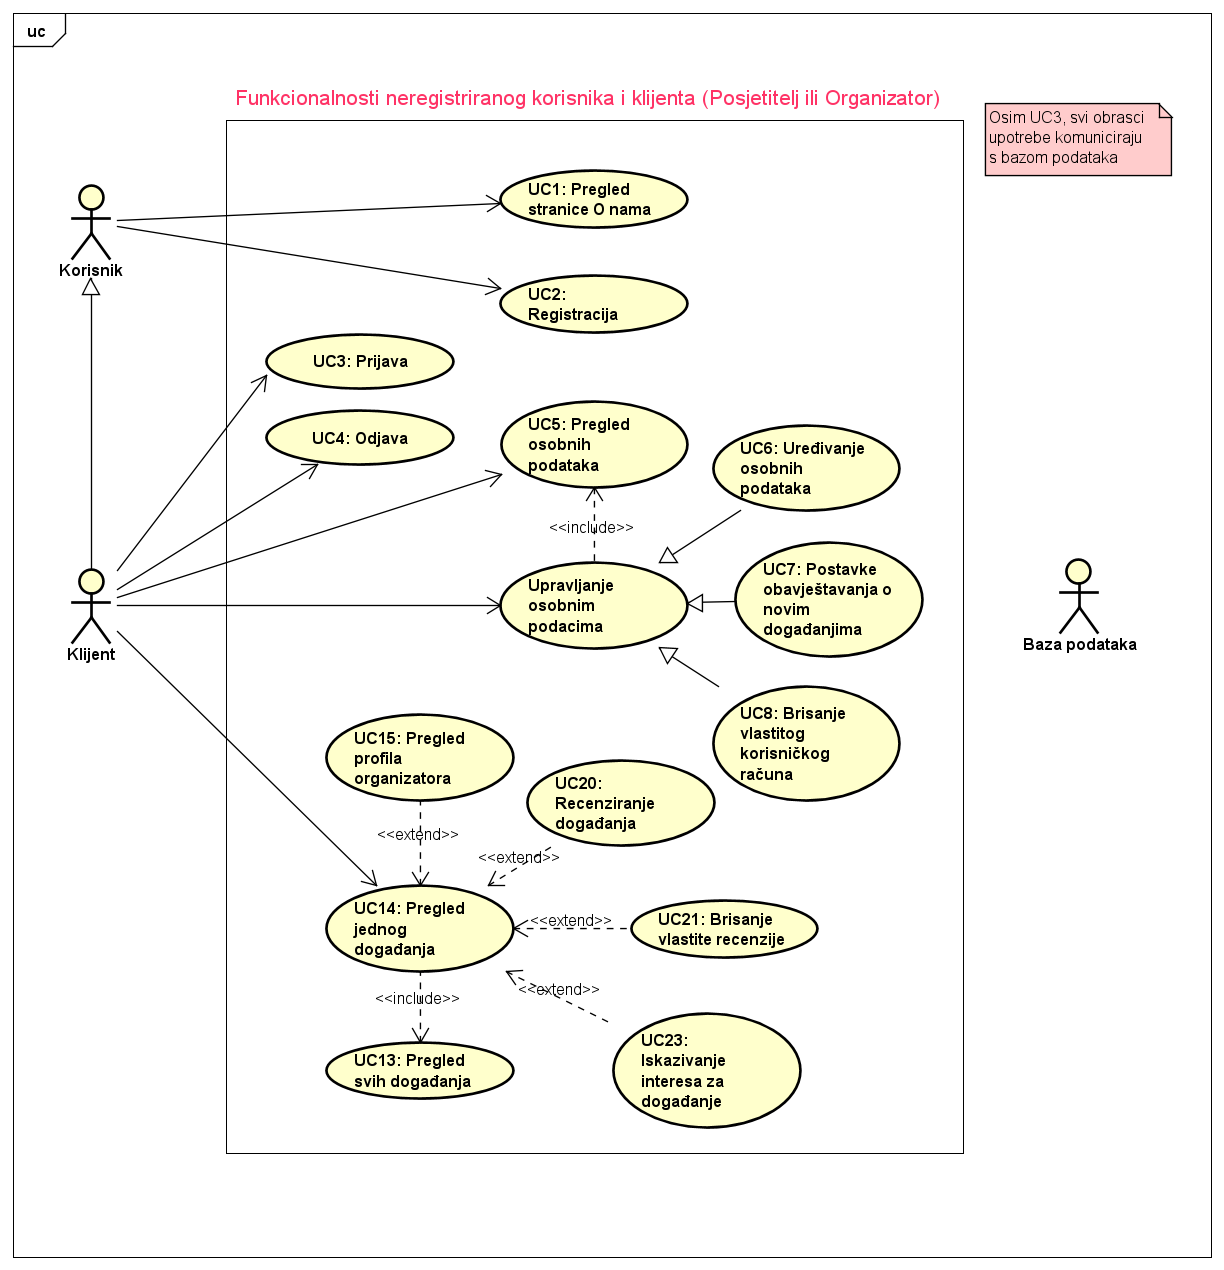
\includegraphics[scale=0.5]{dijagrami/uc1.PNG} 
		\centering
		\caption{Dijagram obrazaca uporabe, funkcionalnost Korisnika i Klijenta (Posjetitelj, Organizator)}
		\label{fig:promjene}
	\end{figure}
	
	\newpage
	
	\begin{figure}[H]
		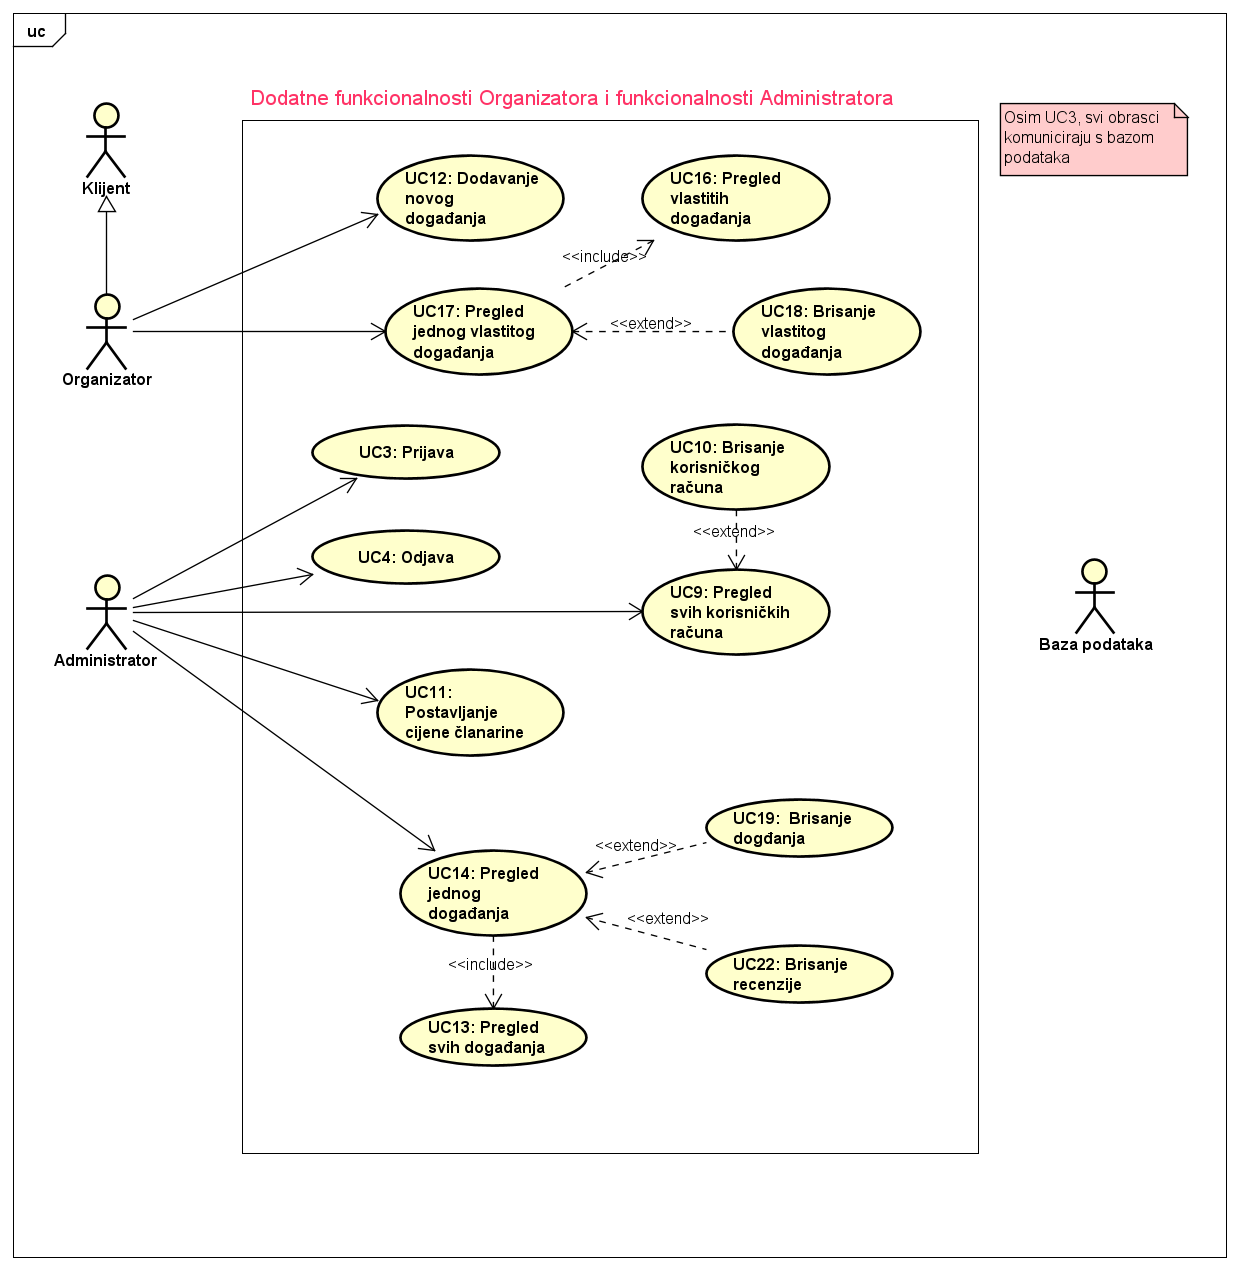
\includegraphics[scale=0.5]{dijagrami/uc2.PNG}
		\centering
		\caption{Dijagram obrazaca uporabe, dodatne funkcionalnosti Organizatora i funkcionalnost Administratora}
		\label{fig:promjene}
	\end{figure}
	
	\newpage
	
	\subsection{Sekvencijski dijagrami}
	
	\noindent \textbf{Obrazac upotrebe UC12 - Dodavanje novog događanja}
	
	\noindent Organizator odabire opciju dodavanja novog događanja. Prikazuje mu se obrazac za unos podataka o događanju. Po završetku unosa željenih podataka, organizator odabire opciju objave događanja. Provjeravaju se uneseni podaci - ako su ispravni, podaci o događanju spremaju se u bazu podataka i novo je događanje objavljeno, inače se prikazuje obavijest o neispravnosti podataka i organizatoru se omogućuje ponovni unos podataka o događanju. 
	
	\begin{figure}[H]
		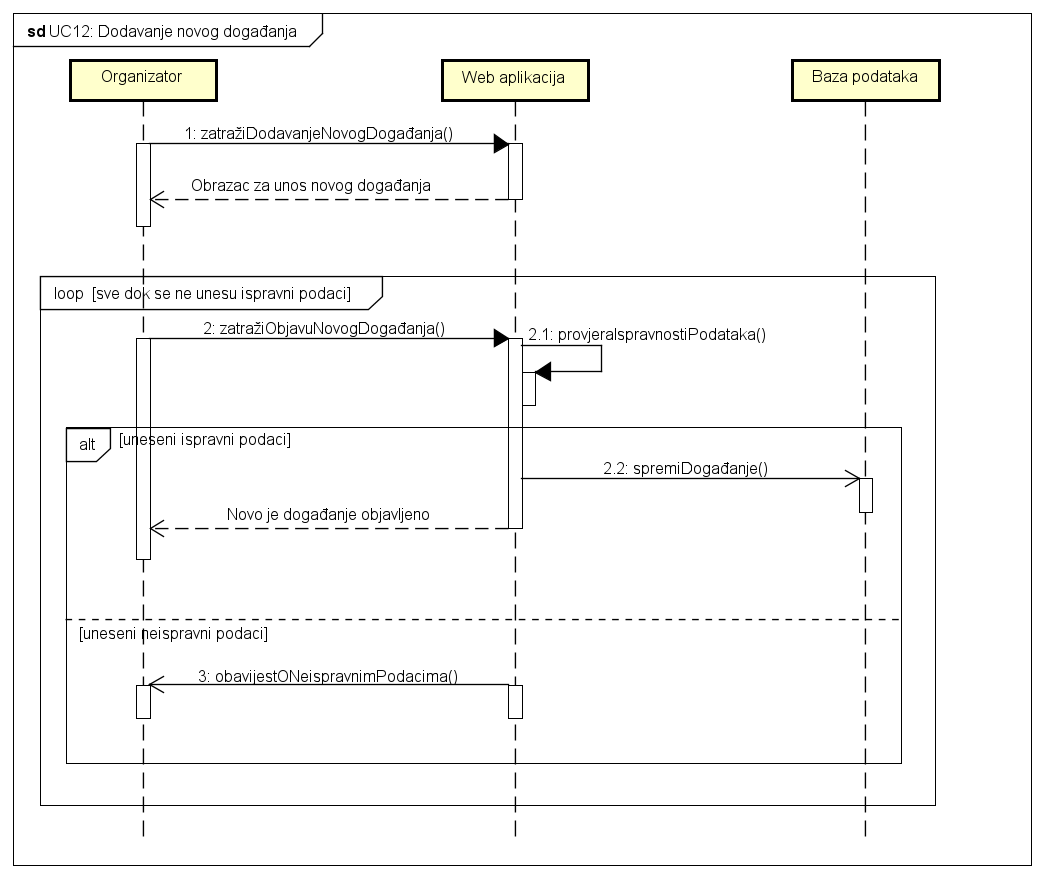
\includegraphics[width=\textwidth]{dijagrami/sd1.PNG}
		\centering
		\caption{Sekvencijski dijagram za \textbf{UC12}}
		\label{fig:promjene}
	\end{figure}
	
	\newpage
	
	\noindent \textbf{Obrazac upotrebe UC20 - Recenziranje događanja}
	
	\noindent Korisnik iz prikaza svih događanja završenih u posljednjih 48 sati odabire jedno koje želi recenzirati. Korisniku se vraća obrazac za unos recenzije. Pri objavi recenzije provjerava se ispravnost recenzije te ako je ispravna, recenzija se sprema u bazu podataka i prikazuje na stranici, u suprotnom korisnik se obavještava o neispravnosti recenzije i istu može napisati ponovno.
	
	\begin{figure}[H]
		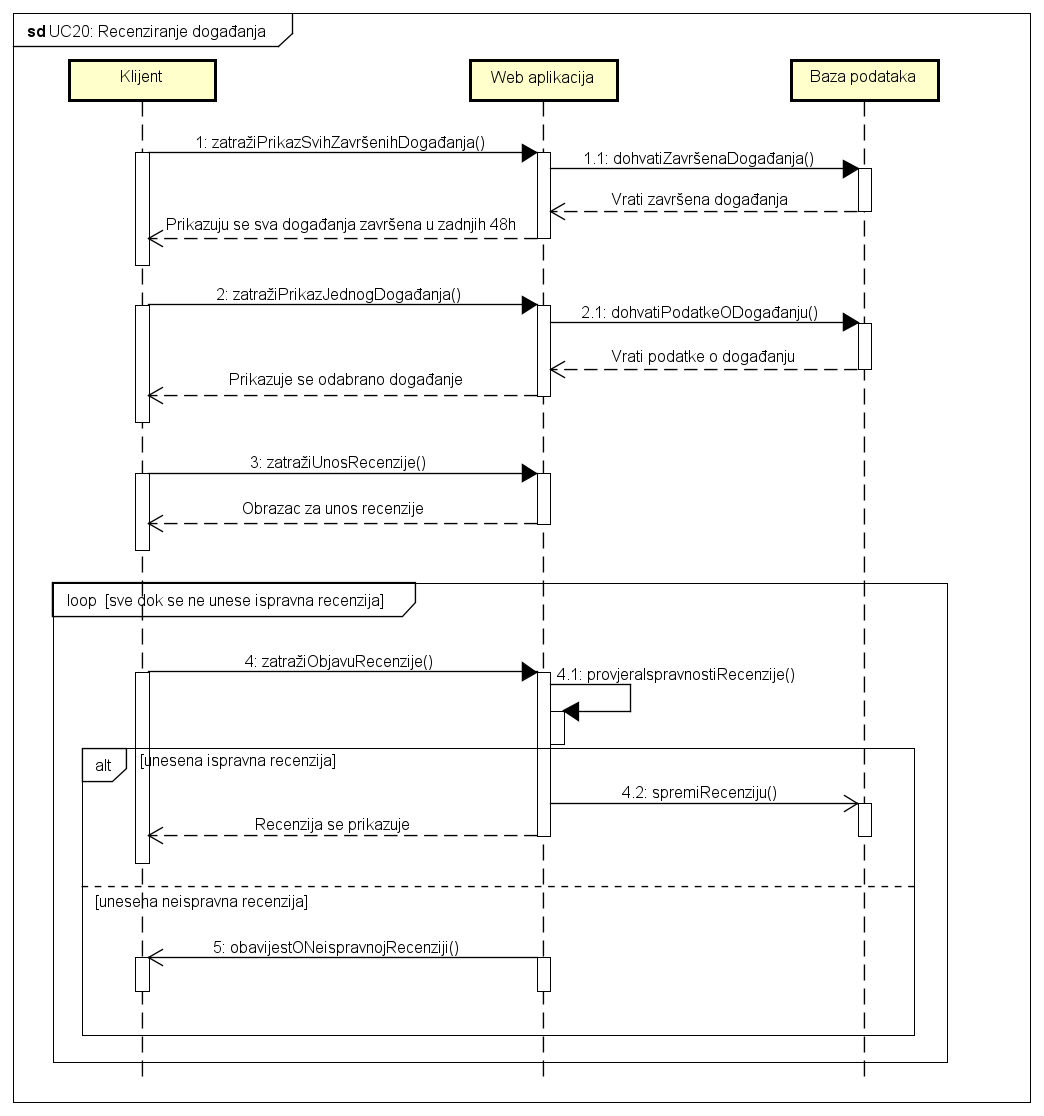
\includegraphics[width=\textwidth]{dijagrami/sd2.PNG}
		\centering
		\caption{Sekvencijski dijagram za \textbf{UC20}}
		\label{fig:promjene}
	\end{figure}
	
	\newpage
	
	\noindent \textbf{Obrazac upotrebe UC23 - Iskazivanje interesa za događanje}
	
	\noindent Korisnik iz prikaza svih događanja završenih u posljednjih odabire jedno za koje želi iskazati interes. Korisniku odabire jednu od opcija \textit{sigurno dolazim}, \textit{možda dolazim}, \textit{ne dolazim}. Obavlja se provjera baze podataka i utvrđuje je li to prvi iskazani interes tog korisnika za događanje ili se radi o promjeni iskazanog interesa. U bazu se sprema novi zapis ili se postojeći mijenja i na stranici korisnik vidi svoj iskazan interes.
	
	\begin{figure}[H]
		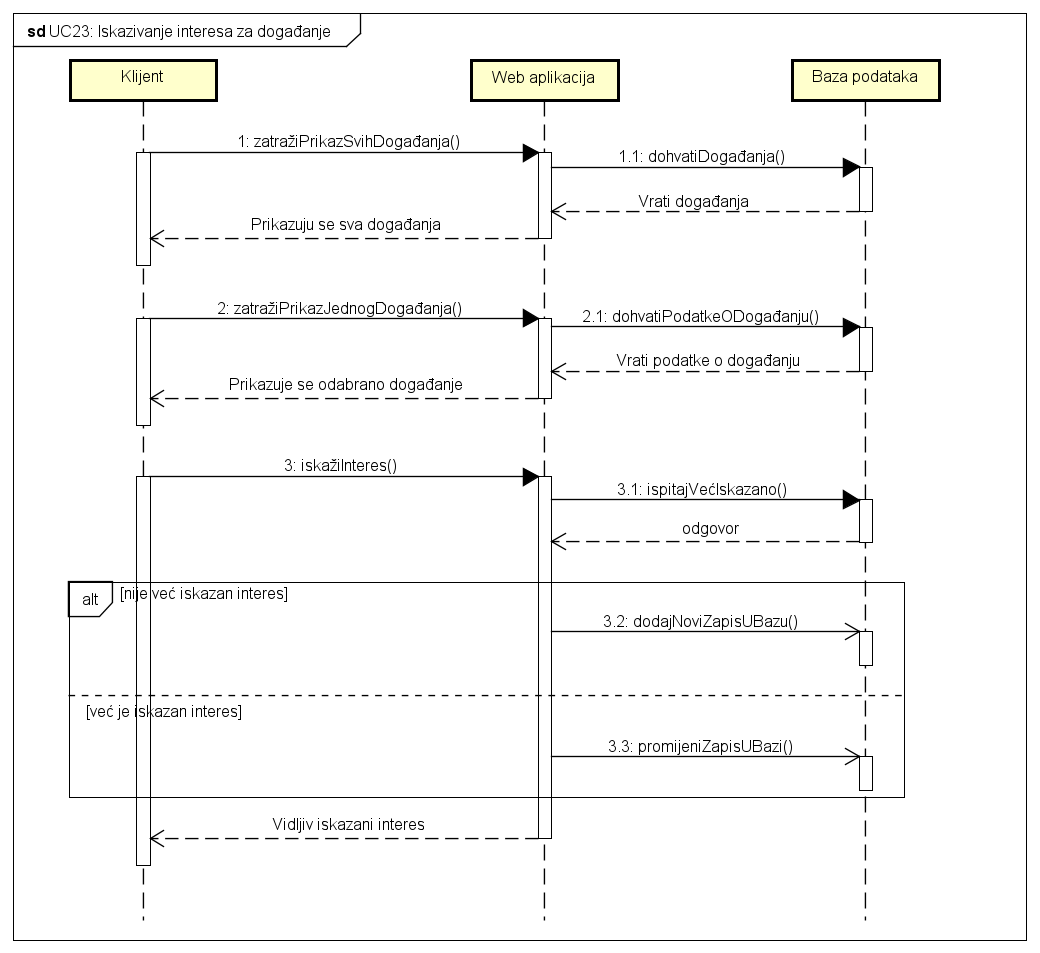
\includegraphics[width=\textwidth]{dijagrami/sd3.PNG}
		\centering
		\caption{Sekvencijski dijagram za \textbf{UC23}}
		\label{fig:promjene}
	\end{figure}
	
	\newpage
	
	\noindent \textbf{Obrasci upotrebe UC9, UC10 i UC11 - Prikaz i brisanje korisničkih računa i postavljanje cijene članarine}
	
	\noindent Administrator odabire opciju prikaza svih korisničkih računa koji se po tom odabiru dohvaćaju iz baze. Kraj korisničkog računa na popisu, administrator može odabrati opciju brisanja korisničkog računa te se brisanje obavlja nakon potvrde. Odabirom opcije za promjenu iznosa članarine administratoru se vraća obrazac u koji administrator unosi novu cijenu članarine sve dok ne unese ispravan iznos.
	
	\vspace{-0.4cm}
	
	\begin{figure}[H]
		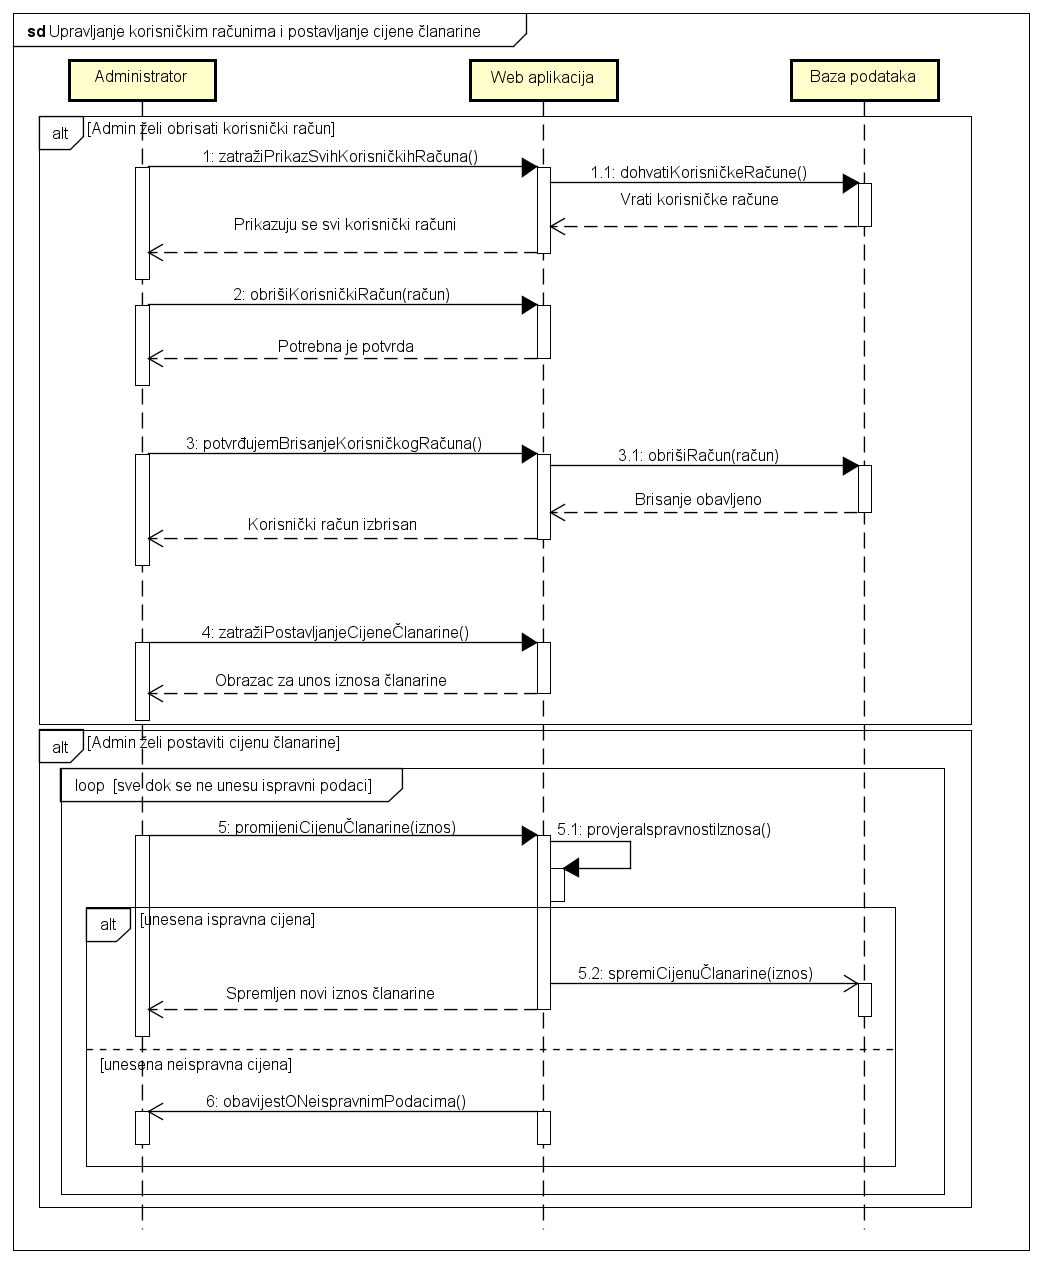
\includegraphics[width=\textwidth]{dijagrami/sd4.PNG}
		\centering
		\vspace{-1cm}
		\caption{Sekvencijski dijagram za \textbf{UC9}, \textbf{UC10} i \textbf{UC11}}
		\label{fig:promjene}
	\end{figure}
	
	\vspace{-0.6cm}
	
	\newpage
	
	\section{Ostali zahtjevi}
	
	\begin{packed_item}
		\item Sustav treba biti implementiran kao web aplikacija koristeći objektno-orijentirane jezike 
		\item Sustav mora omogućiti rad više korisnika u stvarnom vremenu 
		\item Sustav treba sve zadatke izvršavati u vrlo kratkom vremenu, unutar nekoliko sekundi
		\item Korisnički podaci trebaju biti sigurno pohranjeni i odgovarajuće enkriptirani
		\item Sustav mora efikasno pohranjivati, upravljati i pristupati podacima putem baze podataka 
		\item Korisničko sučelje mora podržavati hrvatsku abecedu pri unosu i prikazu tekstualnog sadržaja
		\item Sustav mora koristiti europsku valutu (EUR) za prikaz cijena te europski oblik datuma (\textit{DD.MM.GGGG}) za prikaz i unos datuma
		\item Web aplikacija mora biti responzivna i optimalno korisničko iskustvo pružati na svim uređajima
		\item Korisničko sučelje treba biti intuitivno i pregledno, korisnici se moraju moći koristiti sučeljem bez opširnih uputa
		\item Neispravno korištenje korisničkog sučelja ne smije narušiti funkcionalnosti i rad sustava
		
		
	\end{packed_item}
	
	
